% Chapter 2
\chapter[Experimental approach of surpressing the spectral diffusion]{Sample preparation and Experiment Apparatus} % Main chapter title

\label{Chapter2} % Change X to a consecutive number; for referencing this chapter elsewhere, use \ref{ChapterX}

%----------------------------------------------------------------------------------------
%	SECTION 1
%----------------------------------------------------------------------------------------
\section{Information regarding the nanodiamond sample}

\paragraph{here is a paragraph about the fabrication of nanodiamond}
\FloatBarrier
\begin{figure}[h]
\centering
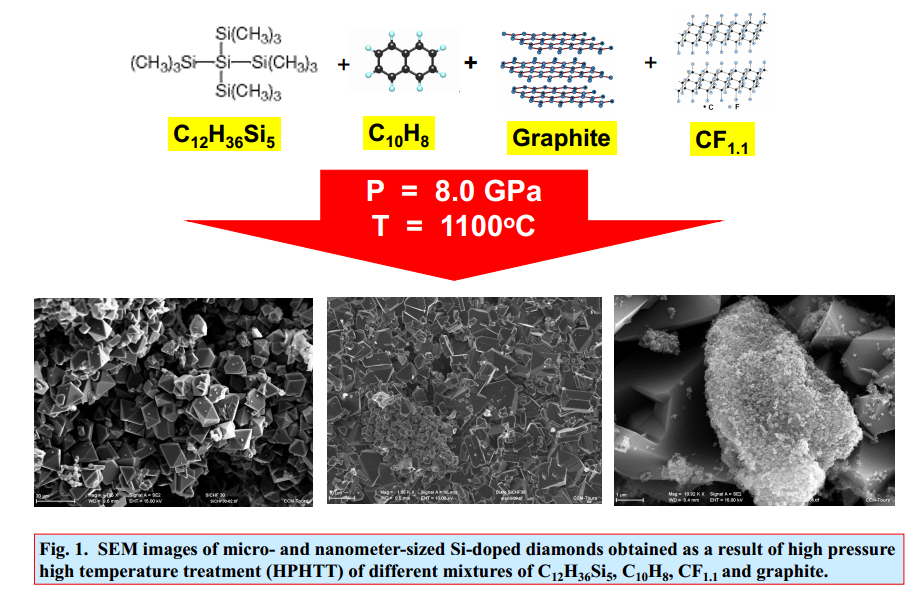
\includegraphics[width=0.7\linewidth]{Figures/pic/Unbenannt}
\caption{}
\label{fig:unbenannt}
\end{figure}
\FloatBarrier

\paragraph{here is a paragraph about the separation of the nanodiamonds}
\FloatBarrier
\begin{figure}[h]
\centering
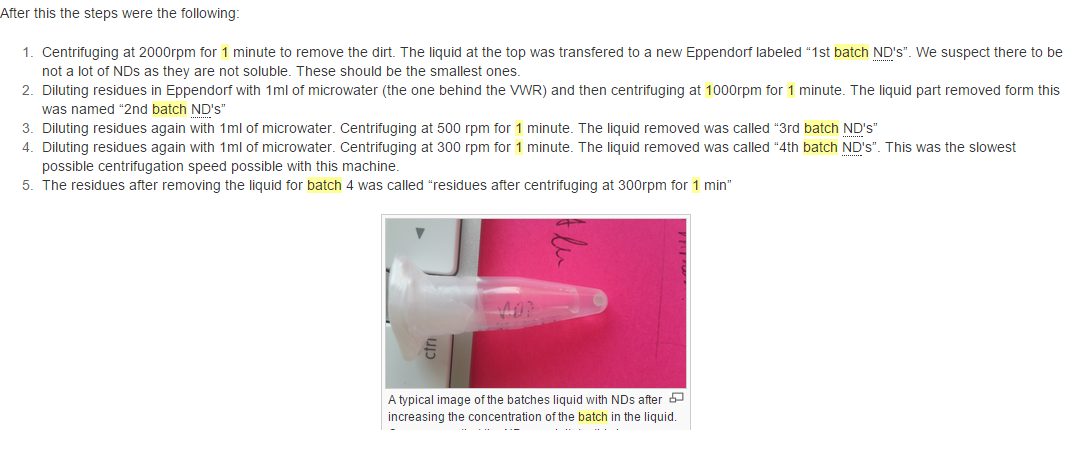
\includegraphics[width=0.7\linewidth]{Figures/pic/Unbenannt1}
\caption{}
\label{fig:unbenannt1}
\end{figure}
\FloatBarrier
\section[sample preparation]{sample preparation}
\subsection{preparation of the substrate}
\paragraph{IIa diamond as substrate}

To choose a proper substrate for the nanodiamond sample, a few principles need to be considered.

\paragraph{1.}Low background fluorescence. 
It is always vital to obtain a decent signal to noise ration in any kind of meansurements. As for our case, the emission(fluorescence) from sillicon centers are the target, thus we would love to lower the back ground fluorescence as much as possilble.
\paragraph{2.}Good heat conductivity at low temperature.
From previous calculation done by Uwen Jantzen, we know that the temperature difference $\bigtriangleup T$ between the bottom of the substrate and nanodiamonds(which are spin coated on the surface of the substrate) can be estimate as\newline
$\bigtriangleup T = \frac{\sigma \cdot d \cdot T^{4}}{k} $,
where $\sigma$ is the Stefan–Boltzmann constant, $d$ is the thickness of the substrate and $k$ is the thermal conductivity.
To resolve the fine feature of sillicon vacancy ZPL, we want to characterise the nanodiamond sample at a temperature that is lower than 30K for spectrometer and 10K? for PLE.
\paragraph{3.} No distracting spectral features.
Some misleading peaks from the emission of the substrate would be the least wanted when we want to character a sample spectrally. In many cases, this is related to the raman-scattering of the photons, which highly depends on the crystal structure of the substrate. This scattering process alters the energy of the incident photons by shifts of concrete values and sometime can introduce peaks that are misleading or distracting.
\paragraph{4.}Refractive index. Inam et al calculated the relative emission rate for radiating dipoles near an interface between two dielectrics with FDTD simulation. The result demonstrates that in both of the cases, when the dipole lies prependicular and parallel to the substrate, the emission rate from a interface with lower relative refractive index is always higher than that from a interface with higher relative refractive index. And to increase the emission rate, a substrate with lower refractive index would be prefered.
\paragraph{}Prevously, taking these principles into consideration, my colleges have already ruled out a couple of materials, for instance, glass/quartz(distraction raman shift lines) and Sapphire(also a distracting raman shift line, and impurity induced emission that calls for extra attention when picking the optical filters). Now the temporary choice has landed on IIa type diamond, which has a low impurity density(resulting in low background fluorescence intensity), relatively low refractive index(2,4 to 2,7), good thermal conductivity($\bigtriangleup T = 4,17 \cdot 10^{-2}K$) and a raman shift at 1332$cm^{-1} $ that causes no distraction on our observation.

\paragraph{Focused Ion Beam milling}
In order to make it more convenient to trace the nanodiamonds, markers were curved onto the surface of the IIa type diamond substrate, this work was done by Uwe Jantzen during his master's thesis period. As is shown in the fig.[], the focues ion beam bombards the surface of diamond away and leaves behind markers that are visible in optical microscopy images and SEM images, as well as confocal microscopy images.
\paragraph{here is a sketch of how Ga-ion bombards the surface of substrate}
\paragraph{here insert image of markers, optical, sem and confocal}
\FloatBarrier
\begin{figure}[h]
\centering
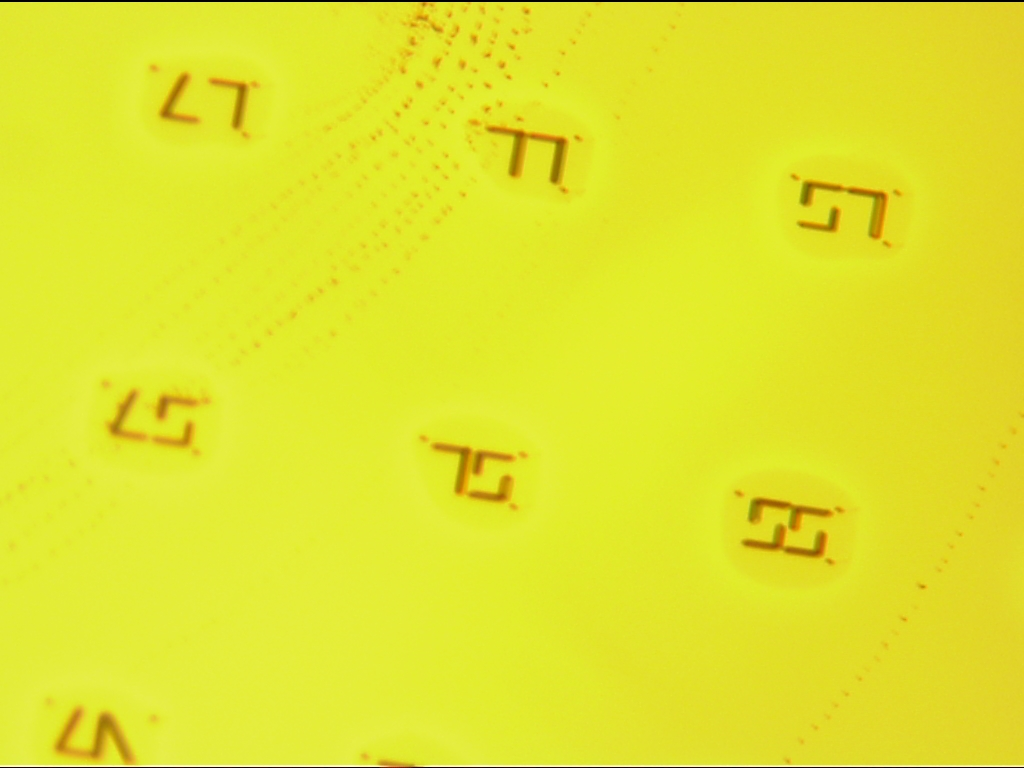
\includegraphics[width=0.7\linewidth]{Figures/pic/20150907_sample214_spincoated_5}
\caption{}
\label{fig:20150907sample214spincoated5}
\end{figure}
\FloatBarrier
\begin{figure}[h]
\centering
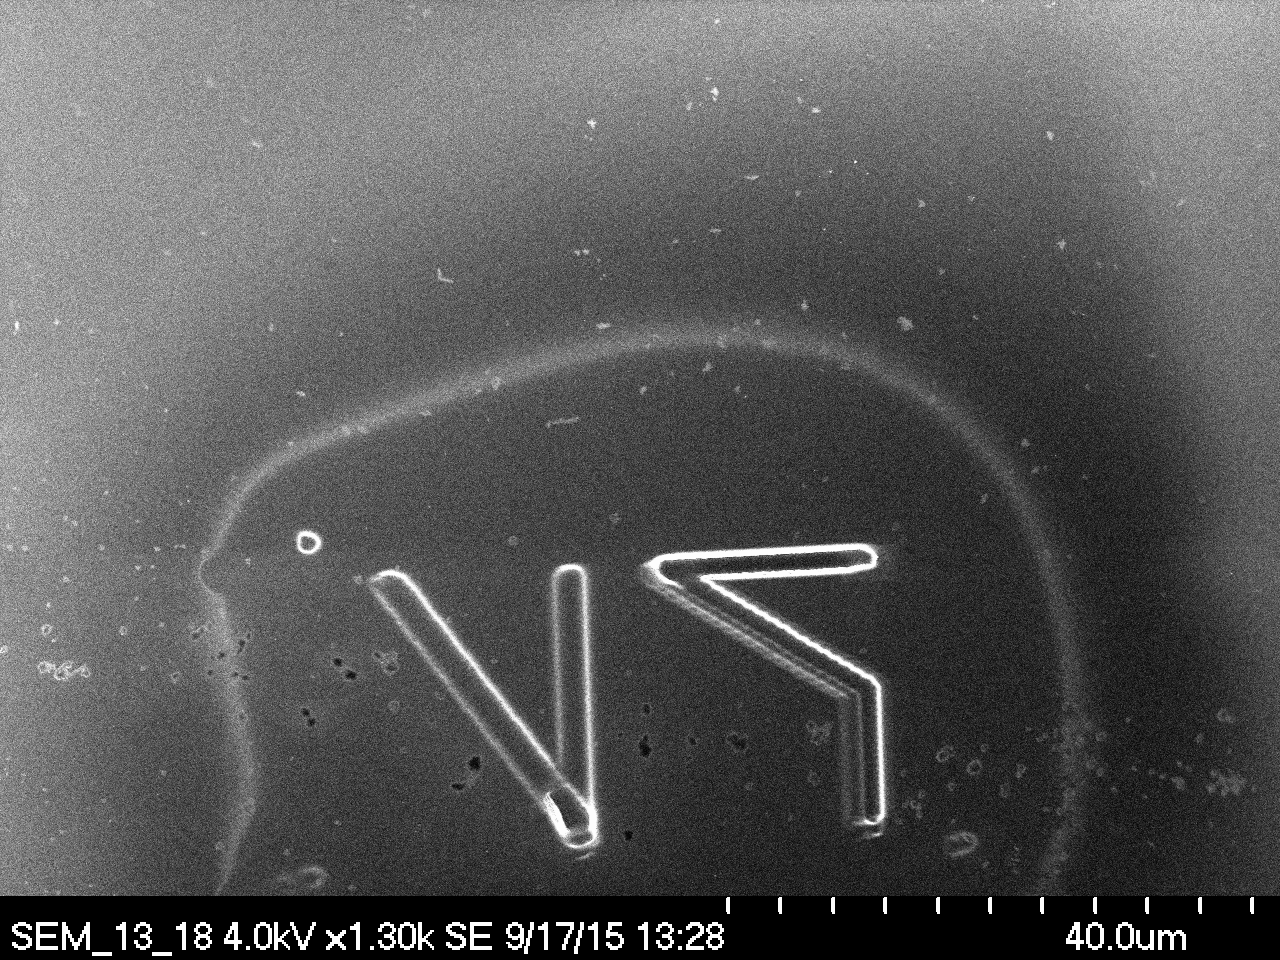
\includegraphics[width=0.7\linewidth]{Figures/pic/20150917-132834_sample214_49_q00}
\caption{}
\label{fig:20150917-132834sample21449q00}
\end{figure}
\FloatBarrier
\begin{figure}[h]
\centering
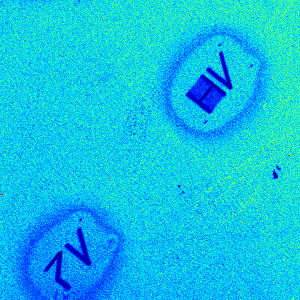
\includegraphics[width=0.7\linewidth]{Figures/pic/2015-09-16_12h06m53s_confocal_xy_image_from_raw}
\caption{}
\label{fig:20150907sample214spincoated5}
\end{figure}
\FloatBarrier


\subsection{spin-coating of the sample}
\subsubsection{theory of spin coating} 
Spin coating is the method of sample preparing that mainly contains 2 steps:

first, the preading of the liquid. In this step, certain volume of liquid containing the particle that we want to coat with is dropped on the surface of the substrate, driven by the centrifuging force from the rotational movement of the substrate, the liquid would be spread evenly on the surface.

Next, the evaporation of the 'solvent'. While the sample stage rotates, the 'solvent'(In our case is not a real solvent, since nanodiamonds never really desolve.) would evaporate, leaving the particle/molecules that are wanted to be coated on the substrate.

In this procedure, a few factors we find important.

1.spin speed: generally the thickness of the liquid layer $t$ is proportional to the inverse of the angular velocity $w$ squared t $\sim$ $\frac{1}{\sqrt{\omega}}$, higher speed would help with forming a more uniform layer, yet this also means a smaller volume of solution, which would lead to lower density of nanodiamonds of the surface. On the other hand, with lower speed, the probability of aggregation would increase, which is also what we want to prevent.

2.volume of the 'solution': larger volume means longer drying time, which would increase the probability of aggregation and losing nanodiamonds, while smaller volume leads towards lower density of nanodiamond and more difficulty when trying to drop it with a pipette. 

3.type of solvent: The type of solvent, viscosity and boiling point are important for the dispersion of nanoparticles inside solution, the spreading of the solution while spin coating and the rate of evaporation.

4.surface condition of the substrate. High contact angle is a obstacle towards the spreading of the solution, high roughness or inappropriate surface group of the substrate can result in poor wettability from the solution.

Additionally, I want to emphasize that, when choosing the spin coating method, the properties of the nanoparticles is always one of the most important thing to take into consideration. 
Throughout my project, with the help of Andrea Kurz, several combination of these factors had been has been tried out:

1. 
2.
3.

\paragraph{here we need a list of different program of spin coating that we have tried,with indexxxxx}

%-----------------------------------
\subsubsection{Acid cleaning}
To make sure that the NDs dispension can evenly spread and eventually settled on the substrate, a smooth, clean and hydrophilic surface is important.

Acid boiling is a very practicle way of diamond substrate cleaning. As it is called, the diamond will be boiled in a mixture of three strong mineral acids: sulfuric acid, nitric acid and perchloric acid. This mixture has ver strong ability of oxidizing.

\paragraph{here insert a sketch of how we do acid cleaning} 

After assembling the setup, we initialize the reaction by heating the mixture to a temperature where is mildly bubbles. The substrate would be stay inside the boiling tri-acid mix for 4h. 
The mixture of strong mineral oxidizing acid can remove most of the adhesions on the surface of diamond substrate , leaving a clean hydrphilic surface. This oxidizing procedure will lead to the formation of carbonyl and carboxyl groups.




\paragraph {here insert image of before and after cleaning substrate, optical image, confocal image }
\FloatBarrier
\begin{figure}[h]
\centering
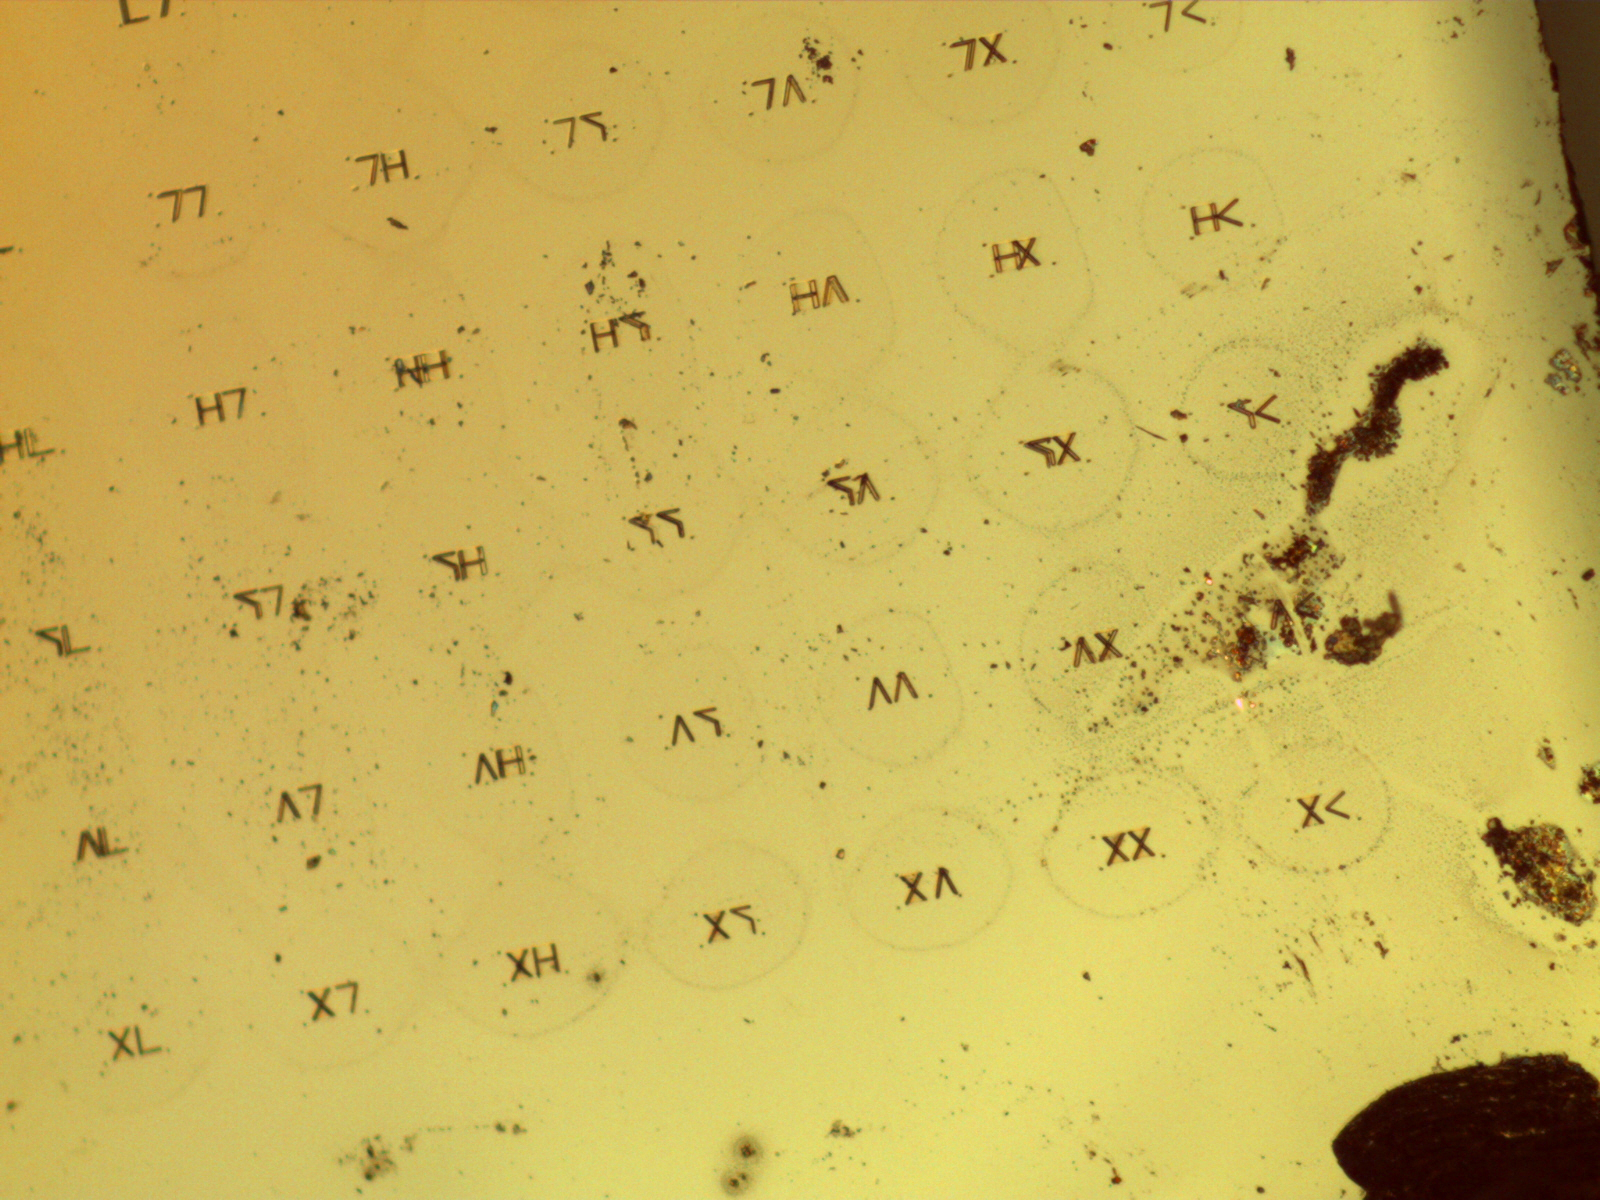
\includegraphics[width=0.7\linewidth]{Figures/pic/image470}
\caption{}
\label{fig:image470}
\end{figure}
\FloatBarrier
fig. the comparision between before and after acid boiling(need to be inserted later).
 

%-----------------------------------
%	SECTION 2
%-----------------------------------
\section[experiment apparatus]{Experiment Apparatus}

\paragraph{The initial Setup} 

The setup can be coarsely separate into laser source, confocal microscope(with APD and spectrometer as detector), flow cryostat and vaccum pump 4 parts.

\begin{figure}[h]
\centering
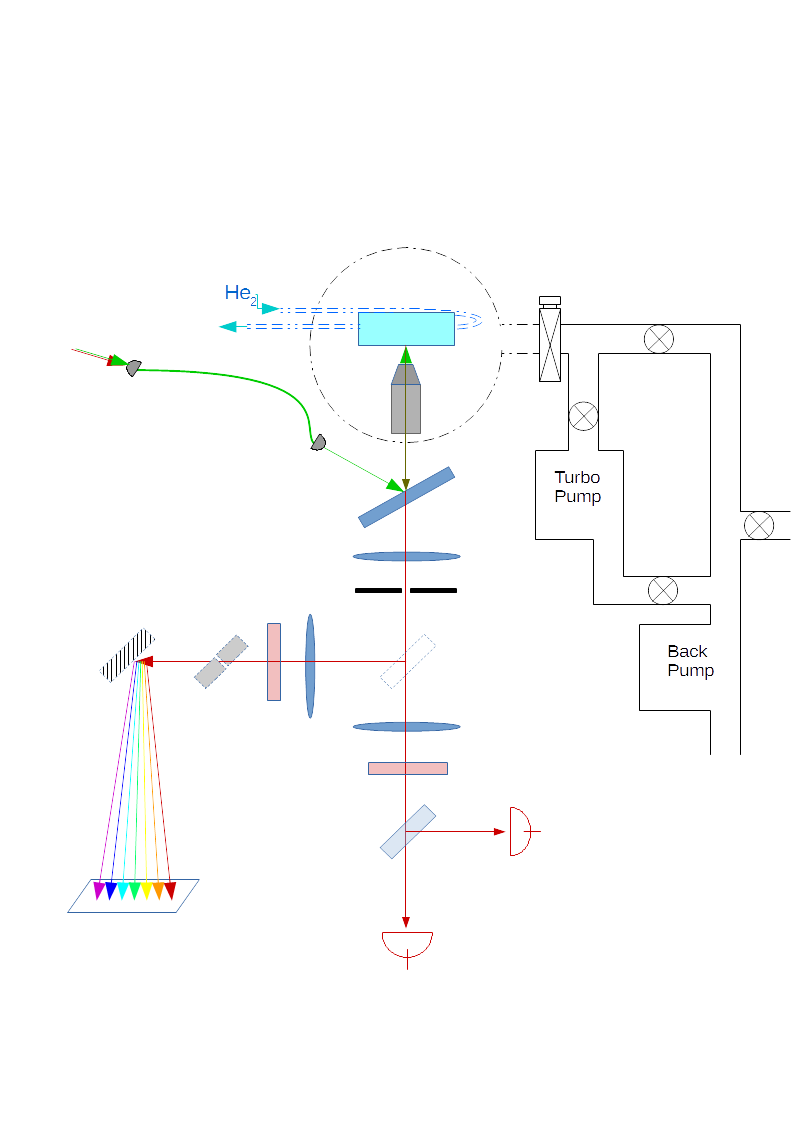
\includegraphics[width=0.7\linewidth]{Figures/pic/initialsetup}
\caption{}
\label{fig:initialsetup}
\end{figure}

Following the optical path, we start from the first part, the laser source.

As has been mention almost countless times, silicon vacancy is our focus of investigation. While the absorption spectrum shows the highest off resonance absorption around 530nm[need check need find reference paper], the ZPL of silicon vacancy lies around 737nm. Acknowledged of such information, we choose to use green laser of wavelength 532nm as the laser source for photoluminesence spectrum and Titan Sapphire laser with the ability of scanning around 737nm as the laser source of photoluminescence excitation. These two methods will be more detailed written about in the following paragraphs.
The lasers are coupled into the same photonic crystal fibre, which guides the beam towards the optical table.

The second part is the confocal microscope, which is a very useful tool for imaging of samples that emits fluorescence, such as SiVs. Compared with fluorescence microscope, the confocal microscope uses a pair of convex lens and a pinhole that conjugates to the lens to achieve the increase of resolution and signal to noise ration.(expend)
In the setup, there are two possibilities of signal detection, controlled by a flipping mirror, we can choose to count the photons with a pair of APD, or record the spectrum with a spectrometer.
\begin{figure}[h]
\centering
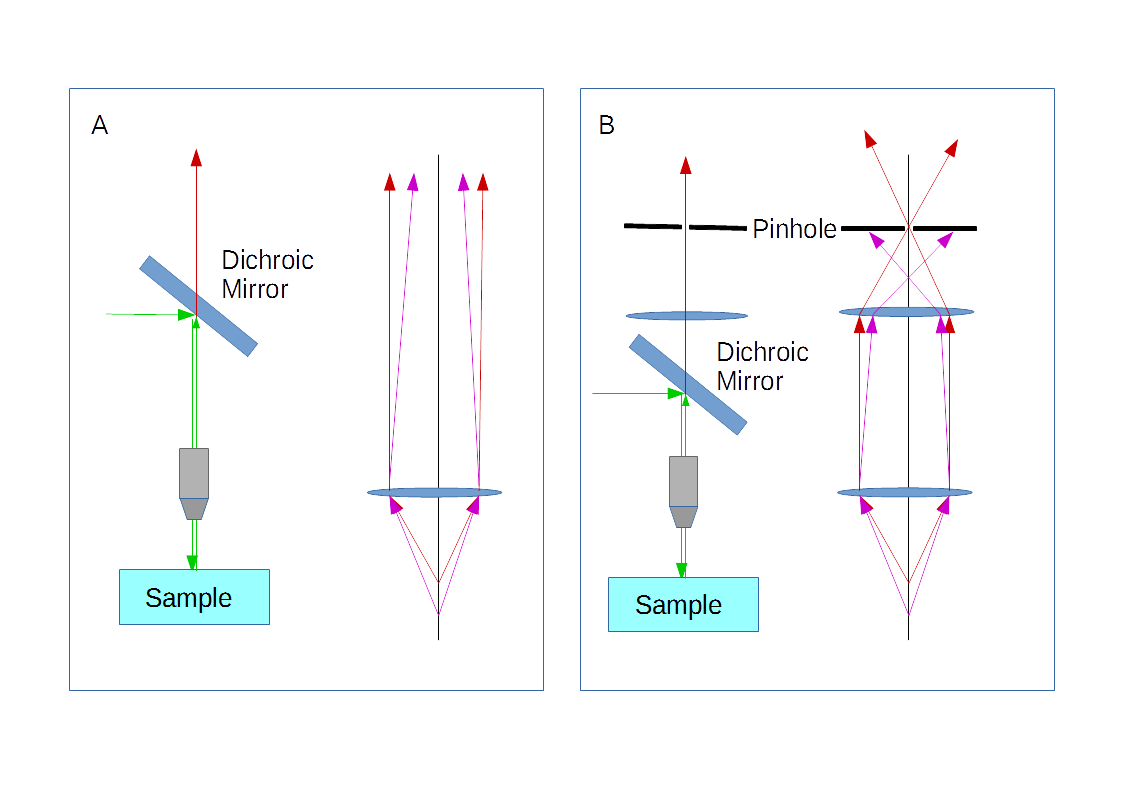
\includegraphics[width=0.7\linewidth]{Figures/pic/microscope}
\caption{}
\label{fig:microscope}
\end{figure}

As the resolution of fine splitting of SiV ZPL needs to be measured in low temperature, the motorized sample stage is placed in a flow cryostat, the objective lens is also inside the cryostat. As the name mentioned, the decrease of temperature in this cryostat is achieved by the flow of cold, boiling liquid Helium, a transfer line connects the Helium dewar and the inlet of the helium cooling circulation inside the cryostat. The sample sits right on the cold finger, with proper method of mounting and substrate, the temperature can be brought to as low as 3.5K(need to check).

To reach cryogenic temperature, it is vital to cut off the heat exchange between the sample and the world out side the cryostat, since air and stainless steel(the material of the cryostat wall) can both conduct heat, a UHV condition need to be meet. In our setup, it is realized by the pumping system of a back pump and a turbo pump. The back pump pre-pumps the pressure until it meets the working condition for turbo pump.

Starts


\paragraph{PL} Photoluminescence spectra is one of the most efficient way of finding silicon vacancies. In this measurement, we use green laser of 532nm to excite the Silicon vacancies from ground state to 

\paragraph{PLE} resonance excitation of optical transition. Rsésolution limited by scanning step of laser. Observing phonon side band with apd. range of scanning: limited by laser, small.

\paragraph{time resolved PL spectra} Tracing PL spectra over time, show the diffusing behaviour of lines, characterisation methods: excitation polarisation: width of diffusion. Cross- correlation over time.
\paragraph{}We recorded and noticed that the diffusion, whose range can up to 1nm, is far beyond the capability of PLE. 